\documentclass{article}
\usepackage[T2A]{fontenc}
\usepackage[utf8]{inputenc}
\usepackage[russian]{babel}

\title{Сравнение алгоритмов построения минимального остовного дерева}
\author{Глеб Пособин}
\date{Декабрь 2014}

\usepackage{natbib}
\usepackage{graphicx}

\begin{document}

\maketitle

\begin{figure}[h!]
\centering
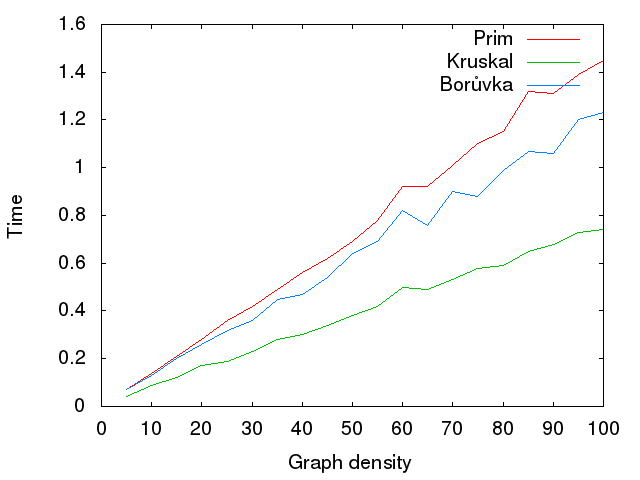
\includegraphics[width=1.0\textwidth]{Graphs.png}
\caption{Время работы трёх алгоритмов на случайных графах из тысячи вершин.}
\label{fig:performance_plot}
\end{figure}

На случайных тестах алгоритм Краскала оказался самым быстрым, а алгоритм Прима --- самым медленным, хотя и не сильно медленнее алгоритма Борувки.
Судя по результатам, у алгоритма Краскала константа, скрытая в асимптотике, в полтора--два раза меньше, чем у двух других алгоритмов.
Ясно, что в таком случае на практике выгоднее использовать алгоритм Краскала.

\end{document}
